\section{NP Completeness}
Boils down to if a problem is solvable in polynomial time or non-deterministic polynomial time.
The mindset I have for this is best describes via excercise 2 from week \emph{NP Completeness}.
\subsection{Example - Customer Uniqueness (KT 8.2)}

A store trying to analyse the behavior of its customers will often main a
two-dimensional array $A$, where the rots correspond to its customers and the
clumns correspond to the products it sells. The antry $A[i,j]$ specifies the
quatity of project $j$ that has been purchaed by customer $i$. 

Here's a tiny example of such an array $A$

\begin{table}[H]
    \centering
    \begin{tabular}{c|c|c|c|c}
        & luquid detergent & beer & diapers & cat litter \\
        \hline
        Raj & 0 & 6 & 0 & 3 \\
        \hline
        Alanis & 2 & 0 & 0 & 7 \\
        \hline
        Chelsea & 0 & 0 & 0 & 7 \\
    \end{tabular}
\end{table}
One thing that a store might want to do with this data is the following. LLet us say that a subset $S$ off the customers is \emph{diverse} if no two of the customers in $S$ have ever bought the same product (i.e., for each product, at most one of the customers in $s$ has ever bought it). A diverse set of customers can be useful, for example, as a target pool for market research.

We can now define the Diverse Subset Problem as follows: Given an $m\times n$ array $A$ as defined abve, and a number $k \leq m$, is there a subset of at least $k$ of customers that is \emph{diverse}?

Show that Diverse subset in NP-complete.
\subsubsection{Solution}
We show that $IS \leq_p DS$, where $IS$ is Independent Set and $DS$ is Diverse Subset. 

Given a graph $G = (V, E)$ with $|V| = m$ vertices and $|E| = n$ edges,
construct an $m \times n$ matrix $A$ where vertices are customers (rows) and
edges are products (columns). For each edge $(u,v) \in E$, set $A[u, (u,v)] =
1$ and $A[v, (u,v)] = 1$ (all other entries are 0).

Now $G$ has an independent set of size $k$ if and only if $A$ has a diverse
subset of size $k$. Since the construction takes polynomial time, $DS$ is
NP-complete.

\subsection{List of NP-complete Problems}
\begin{itemize}
    \item Subset Sum
    \item Independent Set $\ostar$
    \item Vertex Cover $\ostar$
    \item Set Cover
    \item Longest Path $\ostar$
    \item Max Cut $\ostar$
    \item 3-coloring $\ostar$
    \item Hamiltonian Cycle $\ostar$
    \item Travelling Salesperson $\ostar$
\end{itemize}

\subsection{Is P = NP?}
\begin{figure}[H]
\centering
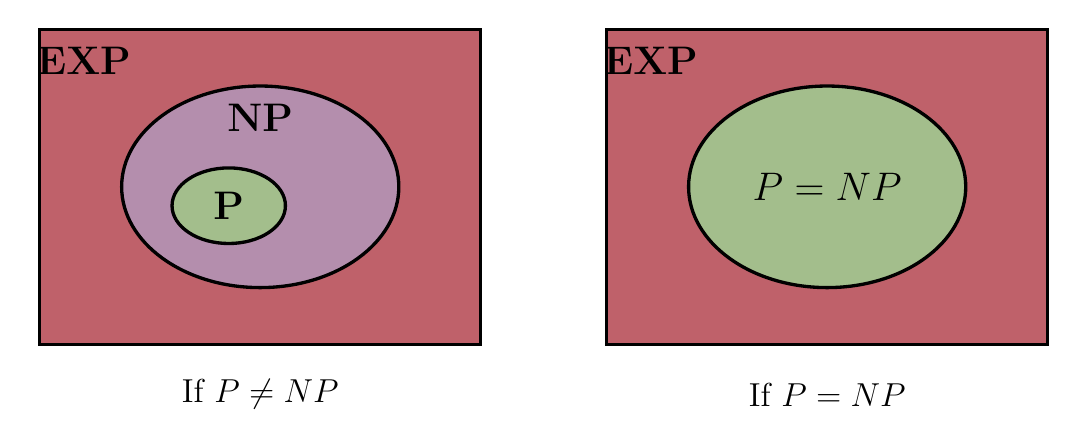
\begin{tikzpicture}[scale=0.8]
    % Define custom colors
    \definecolor{customred}{RGB}{191,97,106}
    \definecolor{custompurple}{RGB}{180,142,173}
    \definecolor{customgreen}{RGB}{163,190,140}

    % Left diagram - If P ≠ NP
    \begin{scope}[xshift=0cm]
        % EXP (box)
        \draw[very thick, fill=customred] (-3.5,-2.5) rectangle (3.5,2.5);
        \node[font=\Large\bfseries] at (-2.8, 2) {EXP};

        % NP (ellipse)
        \fill[custompurple] (0,0) ellipse (2.2cm and 1.6cm);
        \draw[very thick] (0,0) ellipse (2.2cm and 1.6cm);
        \node[font=\Large\bfseries] at (0, 1.1) {NP};

        % P (ellipse)
        \fill[customgreen] (-0.5,-0.3) ellipse (0.9cm and 0.6cm);
        \draw[very thick] (-0.5,-0.3) ellipse (0.9cm and 0.6cm);
        \node[font=\Large\bfseries] at (-0.5, -0.3) {P};

        % Label below
        \node[font=\large] at (0, -3.3) {If $P \neq NP$};
    \end{scope}

    % Right diagram - If P = NP
    \begin{scope}[xshift=9cm]
        % EXP (box)
        \draw[very thick, fill=customred] (-3.5,-2.5) rectangle (3.5,2.5);
        \node[font=\Large\bfseries] at (-2.8, 2) {EXP};

        % P = NP (ellipse)
        \fill[customgreen] (0,0) ellipse (2.2cm and 1.6cm);
        \draw[very thick] (0,0) ellipse (2.2cm and 1.6cm);
        \node[font=\Large\bfseries] at (0, 0) {$P = NP$};

        % Label below
        \node[font=\large] at (0, -3.3) {If $P = NP$};
    \end{scope}
\end{tikzpicture}
\end{figure}
